\section{校区环境}

北邮现在使用中的校区一共三个,即西土城路校区(海淀区,本部)、沙河校区(昌平区)以及海南校区(仅限玛丽女王海南学院)\footnote{另有西城区小西天校区(校舍)和昌平区宏福校区(接近弃用),目前和大家关系不大,唯有实验课偶尔会去一两次。}。

校本部位于海淀区西土城路10号,面积很小,住宿条件相对较差,但交通便利,对面就是北师大,周围美食众多。目前,大部分大三大四的本科生及多数研究生在本部学习。沙河校区是新生入学的校区,位于昌平区沙河镇南丰路1号,规划面积大概本部三倍(但是实际只建成规划面积的一半多),住宿学习环境好,但比较偏僻,出行不便。校园面积真的小,本部绕一圈仅需10分钟,沙河大概也就20分钟。{\small (不过小也有小的好处,比如说可以7:55起床去上8:00的课。)}

除海南学院外的所有新生都将在沙河校区入学并在这至少读完大一。

\begin{center}
    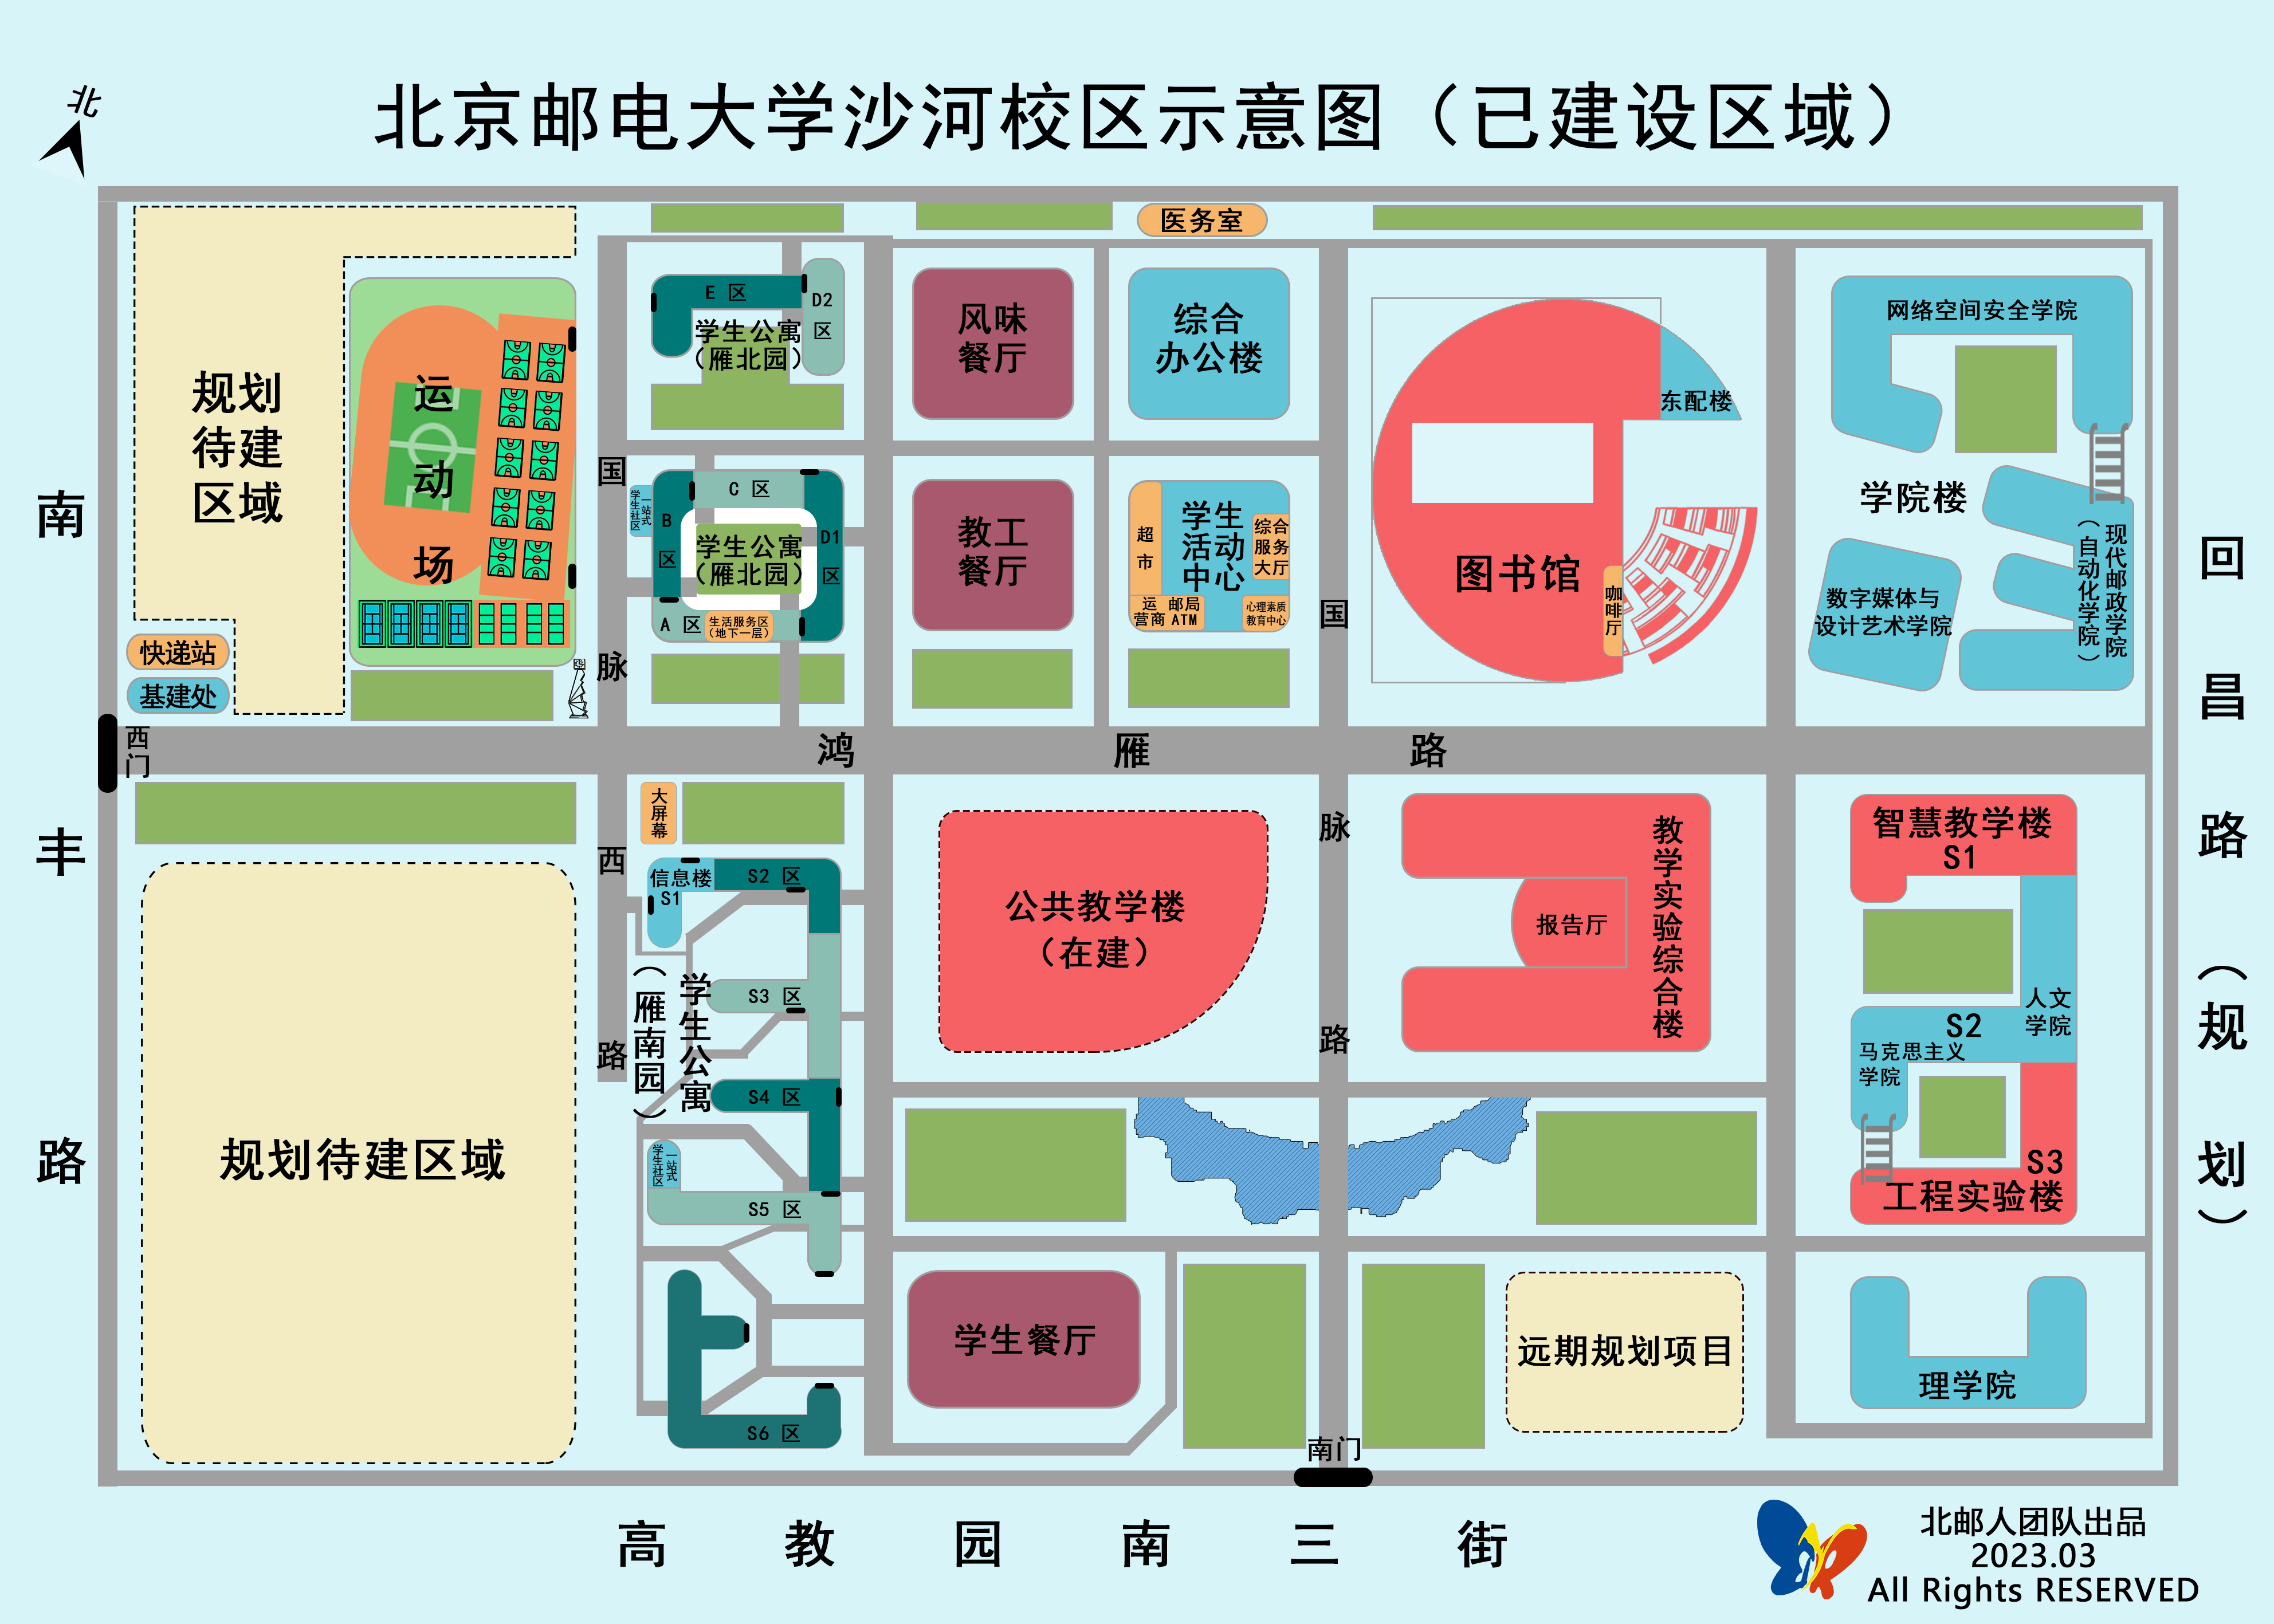
\includegraphics[width=0.80\textwidth]{images/shahe-map.jpg}
\end{center}

\faq{我什么时候会从沙河搬到本部?}

按照学校最新的安排,各个学院的本科生从沙河搬到本部的时间如下表:

\begin{center}
    \begin{tabular}{cc}
        \toprule
        学院 & 搬迁时间(学年开始) \\
        \midrule
        计算机学院(国家示范性软件学院) & 大二 \\
        经济管理学院 & 大二 \\
        国际学院 & 大二\\
        信息与通信工程学院 & 大三 \\
        电子工程学院 & 大三 \\
        人工智能学院 & 大三 \\
        \bottomrule
    \end{tabular}
\end{center}

网络空间安全学院、现代邮政学院(自动化学院)、理学院、人文学院、数字媒体与设计艺术学院不搬至本部(即在沙河校区读完本科四年)。未来学院是否搬至本部、哪学年搬尚不确定。

除参照上表外,学校已经在\href{https://zsb.bupt.edu.cn/info/1005/1992.htm}{招生章程}中写出了各专业的办学地点。

\faq{寒暑假我可以住在学校吗?}

可以住在学校,但由于本科生从沙河校区搬往本部是在新学年开始时进行,所以下一学年搬往本部的同学,暑假只能住在沙河校区。
